\documentclass[12pt]{article}
\documentclass[12pt]{article}
\usepackage[utf8]{inputenc}
\usepackage[spanish]{babel}
\decimalpoint
\usepackage{amsmath}
\usepackage{amsthm}
\usepackage{amssymb}
\usepackage{graphicx}
\usepackage[margin=0.9in]{geometry}
\usepackage{fancyhdr}
\usepackage[inline]{enumitem}
\usepackage{float}
\usepackage{cancel}
\usepackage{bigints}
\usepackage{color}
\usepackage{xcolor}
\usepackage{listingsutf8}
\usepackage{algorithm}
\usepackage{tocloft}
\usepackage[none]{hyphenat}
\usepackage{graphicx}
\usepackage{grffile}
\usepackage{tabularx}
\usepackage[nottoc,notlot,notlof]{tocbibind}
\usepackage{times}
\usepackage{color}
\definecolor{gray97}{gray}{.97}
\definecolor{gray75}{gray}{.75}
\definecolor{gray45}{gray}{.45}
\renewcommand{\cftsecleader}{\cftdotfill{\cftdotsep}}
\pagestyle{fancy}
\setlength{\headheight}{15pt} 
\lhead{Operaciones con cadenas}
\rhead{\thepage}
\lfoot{ESCOM-IPN}
\renewcommand{\footrulewidth}{0.5pt}
\setlength{\parskip}{0.5em}
\newcommand{\ve}[1]{\overrightarrow{#1}}
\newcommand{\abs}[1]{\left\lvert #1 \right\lvert}
\date{22 de febrero de 2018}
\title{Operaciones con cadenas}
\author{Reporte 1}

\definecolor{pblue}{rgb}{0.13,0.13,1}
\definecolor{pgreen}{rgb}{0,0.5,0}
\definecolor{pred}{rgb}{0.9,0,0}
\definecolor{pgrey}{rgb}{0.46,0.45,0.48}
\lstset{tabsize=1}

\usepackage{listings}
\lstset{ frame=Ltb,
framerule=0pt,
aboveskip=0.5cm,
framextopmargin=3pt,
framexbottommargin=3pt,
framexleftmargin=0.4cm,
framesep=0pt,
rulesep=.4pt,
backgroundcolor=\color{gray97},
rulesepcolor=\color{black},
%
stringstyle=\ttfamily,
showstringspaces = false,
basicstyle=\small\ttfamily,
commentstyle=\color{gray45},
keywordstyle=\bfseries,
%
numbers=left,
numbersep=15pt,
numberstyle=\tiny,
numberfirstline = false,
breaklines=true,
}

% minimizar fragmentado de listados
\lstnewenvironment{listing}[1][]
{\lstset{#1}\pagebreak[0]}{\pagebreak[0]}

\lstdefinestyle{consola}
{basicstyle=\scriptsize\bf\ttfamily,
backgroundcolor=\color{gray75},
}

\lstdefinestyle{Java}
{language=Java,
}

%%%%%%%%%%%%%%%%%%%%%

\lstdefinestyle{customc}{
  belowcaptionskip=1\baselineskip,
  breaklines=true,
  frame=L,
  xleftmargin=\parindent,
  language=C,
  showstringspaces=false,
  basicstyle=\footnotesize\ttfamily,
  keywordstyle=\bfseries\color{green!40!black},
  commentstyle=\itshape\color{purple!40!black},
  identifierstyle=\color{blue},
  stringstyle=\color{orange},
}

\lstdefinestyle{customasm}{
  belowcaptionskip=1\baselineskip,
  frame=L,
  xleftmargin=\parindent,
  language=[x86masm]Assembler,
  basicstyle=\footnotesize\ttfamily,
  commentstyle=\itshape\color{purple!40!black},
}

\lstset{escapechar=@,style=customc}

%Permite crear columnas en el documento
\usepackage{multicol} 
\usepackage{color}
\usepackage{comment}
\newcommand{\tabitem}{~~\llap{\textbullet}~~}
\newcommand{\subtabitem}{~~~~\llap{\textbullet}~~}

\bibliographystyle{IEEEtran}
\begin{document}
		\begin{titlepage}
			\begin{center}
				
				% Upper part of the page. The '~' is needed because \\
				% only works if a paragraph has started.
				
				\noindent
				\begin{minipage}{0.5\textwidth}
					\begin{flushleft} \large
						\includegraphics[width=0.3\textwidth]{../ipn.png}
					\end{flushleft}
				\end{minipage}%
				\begin{minipage}{0.55\textwidth}
					\begin{flushright} \large
						\includegraphics[width=0.7\textwidth]{../escom.png}
					\end{flushright}
				\end{minipage}
				
				\textsc{\LARGE Instituto Politécnico Nacional}\\[0.5cm]
				
				\textsc{\Large Escuela Superior de Cómputo}\\[1cm]
				
				% Title
				
				{ \huge Práctica 1 - Operaciones con cadenas \\[1cm] }
				
				{ \Large Unidad de aprendizaje: Teoría computacional} \\[1cm]
				
				{ \Large Grupo: 2CM4 } \\[1cm]
				
				\noindent
				\begin{minipage}{0.5\textwidth}
					\begin{flushleft} \large
						\emph{Alumno(a):}\\
						
						\begin{tabular}{ll}
					     Nicolás Sayago Abigail\\
					\end{tabular}
					\end{flushleft}
				\end{minipage}%
				\begin{minipage}{0.5\textwidth}
					\begin{flushright} \large
						\emph{Profesor(a):} \\
						Sanchez García Luz María  \\
					\end{flushright}
				\end{minipage}
				
				\vfill
				
				% Bottom of the page
				{\large 22 de febrero de 2018}
			\end{center}
		\end{titlepage}
	
	\tableofcontents
		
	\maketitle
	
	\section{Introducción}
	En la siguiente práctica se desarrollaran las operaciones básicas de las cadenas que pertenecen a 
	cierto lenguaje establecido. El lenguaje de programación en el que se desarrolla la práctica es 
	JAVA. Cuenta con una interfaz amigable para el usuario permitiendo ingresar la cadena que el usuario
	desee.

	A lo largo del documento usaremos la palabra \textbf{cadena}, por lo cual tenemos que definir ¿Qué es una cadena? y ¿A qué pertenece?.

	Se llama alfabeto a un conjunto finito, no vacío. Los elementos de un alfabeto se llaman símbolos.
	Un alfabeto se define por la enumeración de los simbolos que contiene. Una palabra o \textbf{cadena} es aquella formada con los símbolos de un alfabeto. Dichas cadenas poseen operaciones y propiedades, que en esta práctica
	se pretenden diseñar e implementar.
	
	Las operaciones básicas de las cadenas son:
	\begin{multicols}{2}
		\begin{itemize}
			\item Longitud
			\item Concatenación
			\item Potencia
			\item Inverso o reflejo
	\breakcolumn
			\item Prefijo
			\item Sufijo
			\item Subcadena
		\end{itemize}
	\end{multicols}
	

	\section{Planteamiento del problema}
	Diseñar la solución para cada una de las operaciones que se pueden hacer con las cadenas:
	\begin{itemize}
		\item Determinar si es palíndromo

		Una palabra es palíndromo si dice lo mismo al derecho
		y al revés, es algo así como: de ida y vuelta. El problema
		es determinar si una cadena es palíndromo.

		Ejemplo: 

		Sea $u$ = ana, entonces $u^{-1}$ = ana. Por lo tanto, la cadena es palíndromo.

		La solución al problema, es usar la operación de invertir la cadena, y compararla
		con la original.

		\item Calculo de Longitud
		
		Se llama longitud de una cadena al número de símbolos que la componen. La longitud de la cadena $x$ se representa con la notación $|x|$ .
		La cadena cuya longitud es cero se llama \textsl{cadena 
		vacía} y se representa con la letra griega $\lambda$.

		En el lenguaje de programación a usar, existe un método que proporciona 
		la longitud de una cadena.

		\item Concatenación de cadenas

		Sean $u$ y $v$ dos cadenas sobre el mismo alfabeto, la 
		concatenación de $u$ y $v$ es una nueva cadena $w$ que se 
		obtiene yuxtaponiendo primero $u$ y detrás $v$, se
		escribe: $w$ = $uv$.

		En el lenjuage de programación a usar, existe un método que permite concatenar las
		cadenas. Evidentemente la concatenación no es asociativa, y el método permite 
		que esta propiedad se cumpla.

		\item Potencias

		Sea $u$ una cadena y $k$ un número entero, definimos:
		\begin{equation*}
			\left.
			\begin{aligned}
			w...^{k)}...w & \text{ \ \ si \ \ } k>0 \\
			\lambda & \text{ \ \ si \ \ } k=0 \\ 
			w^{-1}...^{-k)}...w^{-1} & \text{ \ \ si \ \ } k<0 
			\end{aligned}
			\right\}
			\quad\text{ $u^{k}$ }
		\end{equation*}

		Se concatena la cadena k veces. Para esto se crean subcadenas, hasta obtener la 
		que queremos.

		\item Inverso o reflejo

		Sea $u$ una cadena sobre cierto alfabeto. Llamamos inversa o reflejada de la cadena $u$, y la representamos
		por $u^{-1}$, a la cadena obtenial al escribir los 
		símbolos que constituyen la cadena $u$ en orden inverso.
		Si $u$ = $a_{1}, a_{2},$ ... $a_{n}$, su reflejada sería
		$u$ = $a_{n}, a_{n-1},$ ... $a_{2}, a_{1}$.

		Para este punto tenemos dos soluciones, la que he usado es que se crea una nueva
		cadena que es resultado de obtener el último símbolo de la original hasta llegar
		al primero.

		\item Prefijos

		Un prefijo de la cadena $u$ es cualquier cadena que se
		obtiene al eliminar cero o más símbolos del final de $s$.

		La solución es usar un método que obtendrá cierta posición de la cadena original
		para ir concatenando con lo que se va teniendo.

		\item Sufijos

		Un prefijo de la cadena $u$ es cualquier cadena que se
		obtiene al eliminar cero o más símbolos del principio de 
		$s$.

		La solución es usar un método que obtendrá cierta posición de la cadena original
		para ir concatenando con lo que se va teniendo.
		
		\item Subcadenas

		Una subcadena de $S$ se obtiene al eliminar cualquier prefijo y cualquier sufijo de $S$.

		La solución es usar un método que obtendrá cierta posición de la cadena original
		para ir concatenando con lo que se va teniendo. En este caso en particular, se usa la
		misma técnica que en prefijos.

	\end{itemize}

	\newpage
	\section{Diseño de la solución}

	A continuación mostraré el diseño que se tiene para cada una de las operaciones a realizar.

	\begin{itemize}

		\item Calculo de Longitud

		\begin{figure}[H]
	        \centering
	        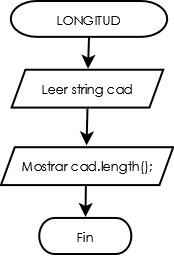
\includegraphics[scale=0.5]{Practica1/Longitud.png}
	    \end{figure}
		
		\item Concatenación de cadenas

		\begin{figure}[H]
	        \centering
	        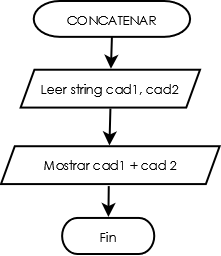
\includegraphics[scale=0.5]{Practica1/Concatenar.png}
	    \end{figure}
	\newpage

		\item Potencias

		\begin{figure}[H]
	        \centering
	        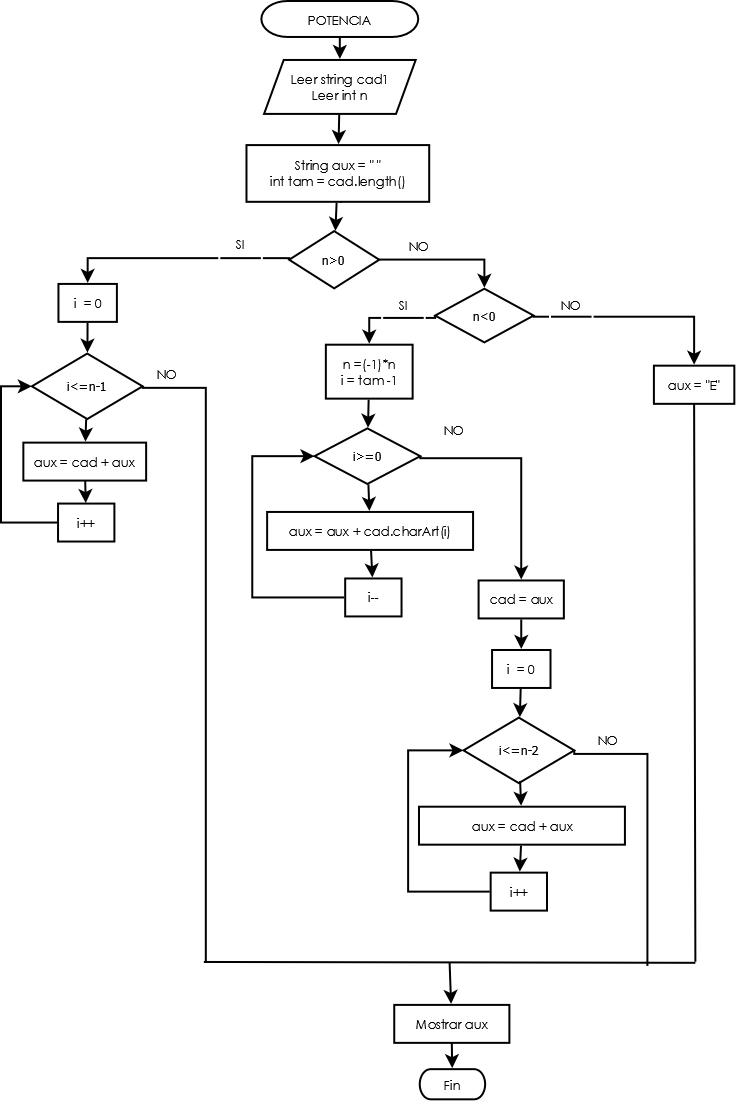
\includegraphics[scale=0.4]{Practica1/Potencia.png}
	    \end{figure}

		\item Inverso o reflejo

		\begin{figure}[H]
	        \centering
	        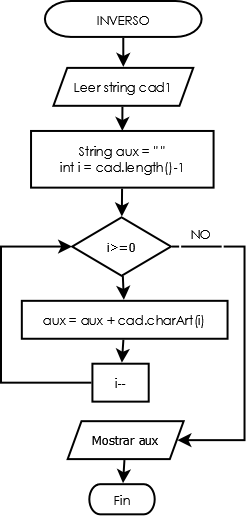
\includegraphics[scale=0.6]{Practica1/Inverso.png}
	    \end{figure}
	\newpage

		\item Prefijos

		\begin{figure}[H]
	        \centering
	        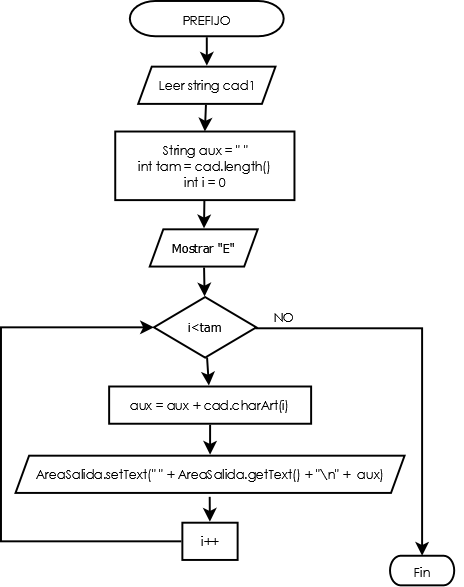
\includegraphics[scale=0.7]{Practica1/Prefijo.png}
	    \end{figure}
	\newpage

		\item Sufijos
		
		\begin{figure}[H]
	        \centering
	        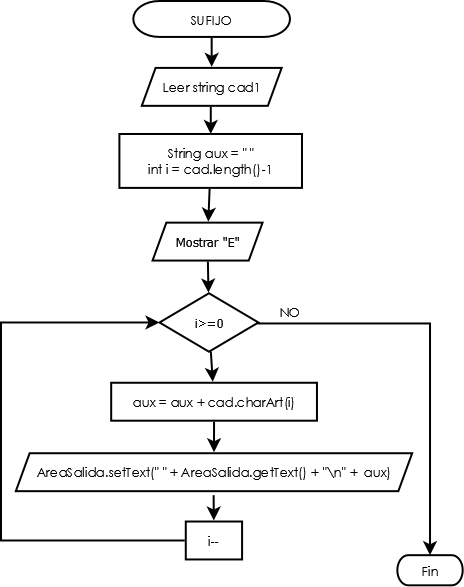
\includegraphics[scale=0.6]{Practica1/Sufijo.png}
	    \end{figure}
	\newpage

		\item Subcadenas

		\begin{figure}[H]
	        \centering
	        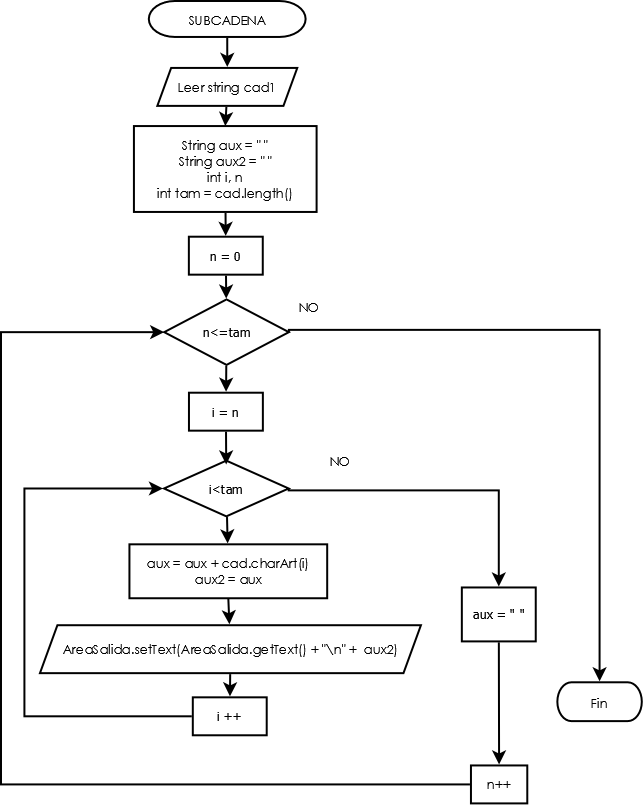
\includegraphics[scale=0.5]{Practica1/Subcadena.png}
	    \end{figure}
	\newpage
	    \item Determinar si es palíndromo
		\begin{figure}[H]
	        \centering
	        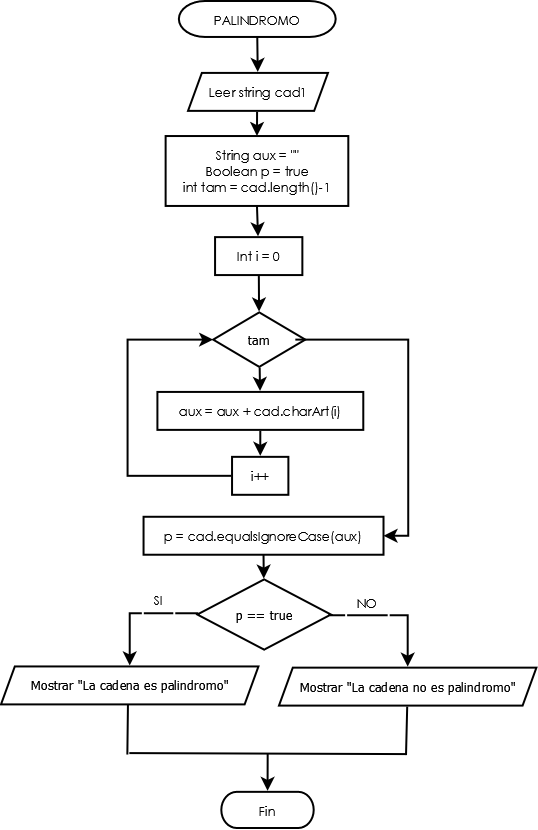
\includegraphics[scale=0.5]{Practica1/Palindromo.png}
	    \end{figure}
	\end{itemize}
	\newpage
	\section{Implementación de la solución}

	El programa consta de 9 métodos de los cuales 8 corresponden 
	a cada una de las operaciones que se requieren. 

	Primero muestro una tabla con los métodos con los que ya cuenta el 
	lenguaje de programación y que fueron utilizados en la realización 
	de las operaciones.

	 \begin{table}[H]
        \begin{tabular}{|p{6.5cm}|p{9.5cm}|}
        \hline
            \textbf{Método} & \textbf{Función} \\ \hline
            cadena.charAr(indice) & Devuelve el caracter que encuentra en una posición especifica. \\ \hline
            cadena.length() & Devuelve la longitud de la cadena tomando en cuenta los espacios. \\ \hline
           	string.equalsIgnoreCase(string2) & Devuelve true si una cadena es igual a la otra y false en caso contrario. \\ \hline
        \end{tabular}
    \end{table}

	
	\begin{itemize}
		\item Determinar si es palíndromo

		\begin{lstlisting}[style=Java]
			public void Palindromo(int sel)
			{
				int i;
				Boolean p = true; // Bandera
				String cad = campos[sel].getText(); //Cadena elegida
				String aux=""; //Cadena auxiliar para guardar el inverso
				//Invertimos la cadena
				for (i = cad.length()-1; i>=0; i--)
					aux = aux + cad.charAt(i); 
				// Comparamos la original con la invertida
				p = cad.equalsIgnoreCase(aux); 
				if(p == true) // Si la bandera no ha sido modificada
					AreaSalida.setText("LA CADENA ES PALINDROMO");
				else 
					AreaSalida.setText("LA CADENA NO ES PALINDROMO");
			}
		\end{lstlisting}

		\item Calculo de Longitud
		\begin{lstlisting}[style=Java]
			public void longi(int sel)
			{
				String cad = campos[sel].getText(); //Obtenemos la cadena
				String mensaje = "LA LONGITUD DE LA CADENA ES: \n\n";
				if (cad.equalsIgnoreCase("E")) // Para la cadena vacía
					AreaSalida.setText(mensaje + "|"+ cad +"|" +" = "+ "0" +"\n"); 
				else // Para cualquier otra cadena
					AreaSalida.setText(mensaje + "|"+ cad + "|" +" = "+ cad.length() +"\n");
			}
		\end{lstlisting}
	\newpage
		\item Concatenación de cadenas
		\begin{lstlisting}[style=Java]
			public void Concatenar()
			{
				String cad1 = campos[0].getText(); //Obtenemos la primera cadena
				String cad2 = campos[1].getText(); //Obtenemos la segunda cadena
				String mensaje = "CONCATENACION DE LA CADENA 1 Y CADENA 2: \n\n";
				AreaSalida.setText( mensaje + "\n\n"+ cad1 + cad2 ); // Se concatenan
			}
		\end{lstlisting}
		
		\item Potencias
		\begin{lstlisting}[style=Java]
			public void Potencia(int sel)
			{
				int tam, i;
				String cad = campos[sel].getText(); // Se obtiene la cadena
				int n = Integer.parseInt(campos[3].getText()); // Se obtiene la potencia
				String aux=""; // Cadena auxilar para guardar la nueva cadena
				tam = cad.length(); // Tamaño de la cadena
				// CASO: La potencia es positiva
				if(n > 0)
				{
					// Concatenamos la cadena consigo misma n veces
					for (i=0; i<=n-1; i++)
						aux = cad + aux;
				}
				// CASO: La potencia es negativa
				else if(n<0) 
				{
					// Invertimos la cadena
					n=-1*n;
					for (i = tam-1; i>=0; i--)
						aux = aux + cad.charAt(i);
					cad = aux;
					// Concatenamos la cadena consigo misma n veces
					for (i=0; i<=n-2; i++)
						aux = cad + aux;
				}
				// CASO: La potencia es 0
				else if(n == 0)
					aux = "E";	// Cadena vacía
				// Se muestra la nueva cadena
				AreaSalida.setText("LA POTENCIA ES:\n\n" + aux +"\n");
			}			
		\end{lstlisting}
	\newpage

		\item Inverso o reflejo
		\begin{lstlisting}[style=Java]
			public void Inverso(int sel)
			{
				String cad = campos[sel].getText(); //Se obtiene la cadena
				String aux=""; // Cadena auxiliar para guardar el inverso
				int i, tam; 
				tam = cad.length(); // Tamaño de la cadena
				//Invertimos la cadena
				for (i = tam-1; i>=0; i--)
					aux = aux + cad.charAt(i);
				// Se muestra la cadena auxiliar
				AreaSalida.setText("LA CADENA INVERTIDA ES:" +"\n\n" + aux);
			}
		\end{lstlisting}
		
		\item Prefijos
		\begin{lstlisting}[style=Java]
		public void Prefijo(int sel)
		{
			int tam, i;
			String cad = campos[sel].getText(); // Obtenemos a cadena
			String aux = "";  // Cadena auxiliar para guardar la nueva cadena
			tam = cad.length(); // Tamaño de la cadena
			AreaSalida.setText("E"); // Se imprime la cadena vacía
			// Se imprimen los prefijos, recorriendo cadda simbolo de la cadena
			for (i=0; i<tam; i++) // Iniciamos del primer simbolo
			{
				aux = aux + cad.charAt(i); //Nueva cadena
				AreaSalida.setText(" " + AreaSalida.getText() + "\n" +  aux);
			}
		}	
		\end{lstlisting}
		
		\item Sufijos
		\begin{lstlisting}[style=Java]
			public void Sufijo(int sel)
			{
				int tam, i;
				String cad = campos[sel].getText(); // Se obtiene la cadena
				String aux = ""; // Cadena auxilar para guardar la nueva cadena
				tam = cad.length(); // Tamaño de la cadena
				AreaSalida.setText("E"); // Se imprime la cadena vacía
				// Se imprimen los sufijos, recorriendo cada simbolo de la cadena
				for(i=tam-1; i>=0; i--) // Iniciamos de último simbolo
				{
					aux = cad.charAt(i) + aux; // Nueva cadena
					AreaSalida.setText(" " + AreaSalida.getText() + "\n" +  aux);
				}
			}
		\end{lstlisting}
	\newpage
		\item Subcadenas
		\begin{lstlisting}[style=Java]
		public void Subcadena(int sel)
		{
			String cad = campos[sel].getText(); // Obtenemos la cadena
			String aux = ""; // Cadena auxiliar para guardar cada subcadena
			String aux2 = ""; // Cadena auxiliar para imprimir cada subadena
			int i, tam, n; 
			tam = cad.length(); // Tamaño de la cadena
			n = 0; // Variable para iniciar desde cierto simbolo
			while(n<=tam) // Para que no se rebase el limite 
			{
				for (i=n; i<tam; i++) // Se inicia en el simbolo indicado
				{
					aux = aux + cad.charAt(i); // Generamos la nueva cadena
					aux2 = aux; // Guardamos en otra cadena para imprimir
					// Mostramos todo lo que ya teníamos y la nueva cadena
					AreaSalida.setText(AreaSalida.getText() + "\n" +  aux2); 
				}
				aux = " "; // Limpiamos la cadena auxiliar
				n++; // Se recorre el indice de inicio
			}
		}			
		\end{lstlisting}
	\end{itemize}
	\newpage
	\section{Funcionamiento}
	Primero que nada, mostramos la interfaz inicial. Observamos que el 
	usuario tiene la oportunidad de ingresar dos cadenas. Y tiene que elegir si quiere ver los resultados de la cadena 1 o 2, unicamente poniendo esos números en el campo correspondiente. Y existe un campo especial para escribir la potencia. Cada botón permite realizar una operación.

	\begin{figure}[H]
	        \centering
	        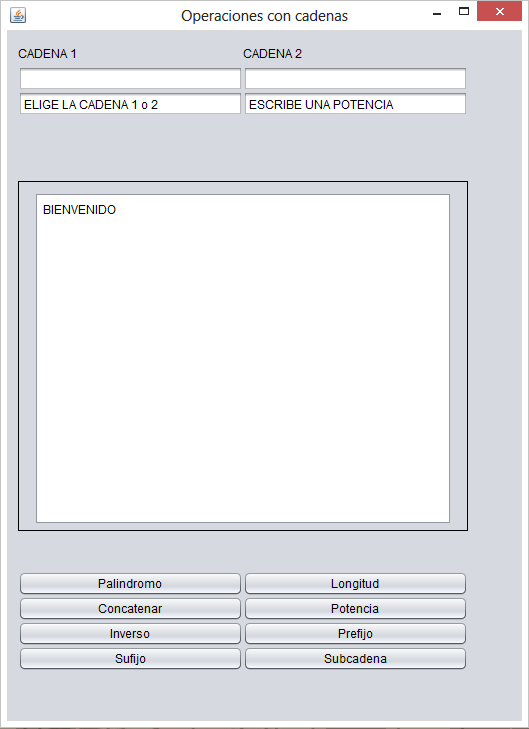
\includegraphics[scale=0.5]{Practica1/Inicio.PNG}
    \end{figure}

	\begin{itemize}

		\item Calculo de Longitud
		
		\begin{figure}[H]
	        \centering
	        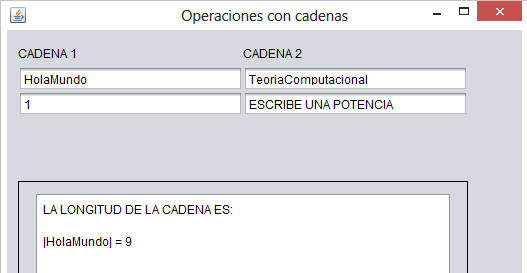
\includegraphics[scale=0.7]{Practica1/Lon_1.PNG}
    	\end{figure}
		\begin{figure}[H]
	        \centering
	        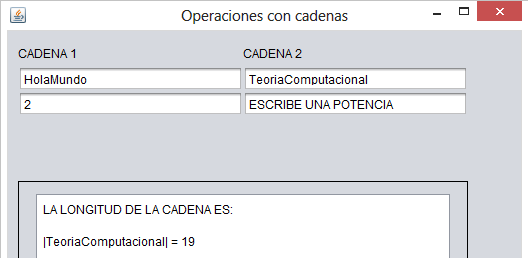
\includegraphics[scale=0.7]{Practica1/Lon_2.PNG}
    	\end{figure}

		\item Concatenación de cadenas

		\begin{figure}[H]
	        \centering
	        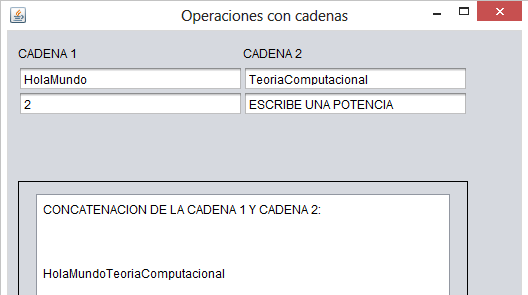
\includegraphics[scale=0.7]{Practica1/Conca.PNG}
    	\end{figure}
    	
		\item Potencias

		\begin{figure}[H]
	        \centering
	        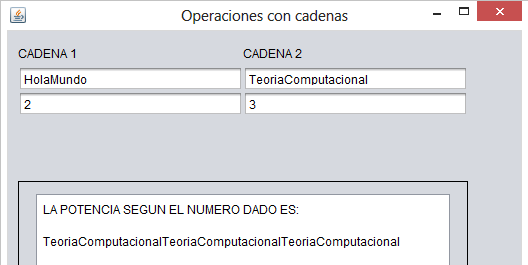
\includegraphics[scale=0.7]{Practica1/Pot.PNG}
    	\end{figure}
    \newpage
		\item Inverso o reflejo
		
		\begin{figure}[H]
	        \centering
	        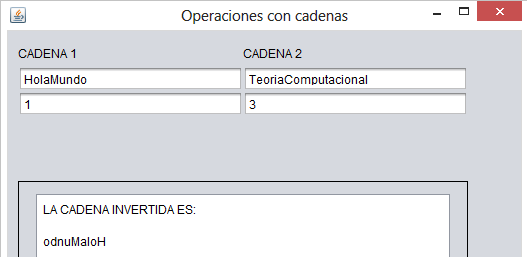
\includegraphics[scale=0.7]{Practica1/Inverso.PNG}
    	\end{figure}
    	
		\item Prefijos
		\begin{figure}[H]
	        \centering
	        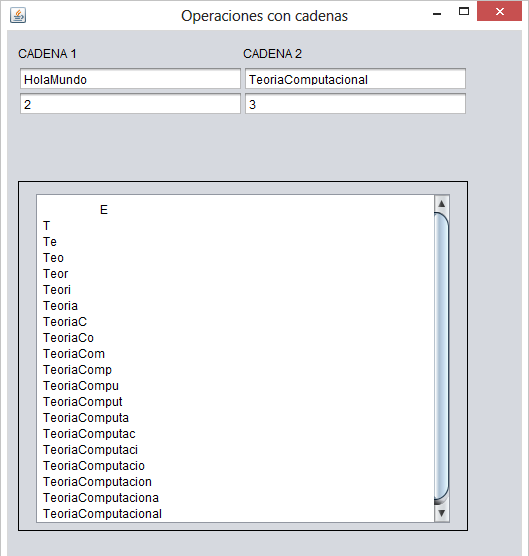
\includegraphics[scale=0.7]{Practica1/Pre_1.PNG}
    	\end{figure}
   	\newpage
		\item Sufijos

		\begin{figure}[H]
	        \centering
	        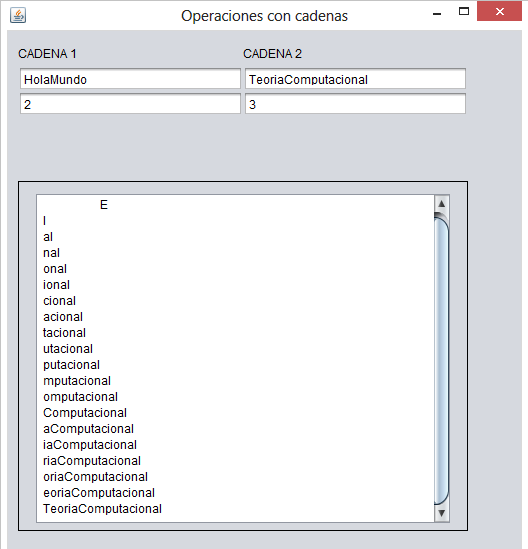
\includegraphics[scale=0.7]{Practica1/Suf_1.PNG}
    	\end{figure}
    	
		\item Subcadenas

		\begin{figure}[H]
	        \centering
	        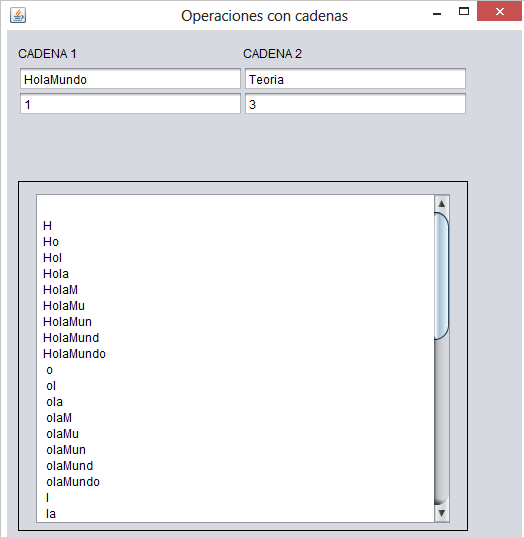
\includegraphics[scale=0.7]{Practica1/Sub_1.PNG}
    	\end{figure}
		\begin{figure}[H]
	        \centering
	        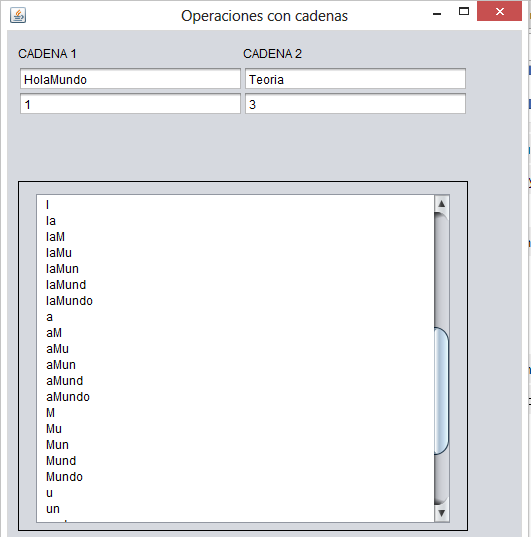
\includegraphics[scale=0.7]{Practica1/Sub_2.PNG}
    	\end{figure}
		\begin{figure}[H]
	        \centering
	        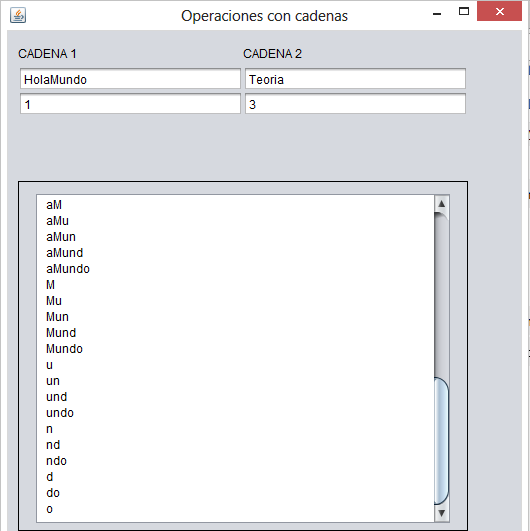
\includegraphics[scale=0.7]{Practica1/Sub_3.PNG}
    	\end{figure}
\newpage
	    \item Determinar si es palíndromo

		\begin{figure}[H]
	        \centering
	        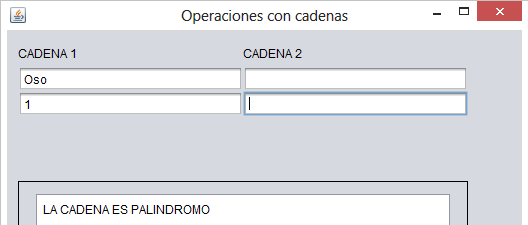
\includegraphics[scale=0.7]{Practica1/Pal_1.PNG}
    	\end{figure}
		\begin{figure}[H]
	        \centering
	        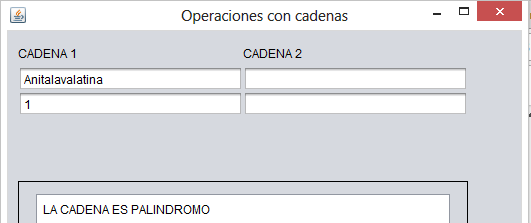
\includegraphics[scale=0.7]{Practica1/Pal_2.PNG}
    	\end{figure}
		\begin{figure}[H]
	        \centering
	        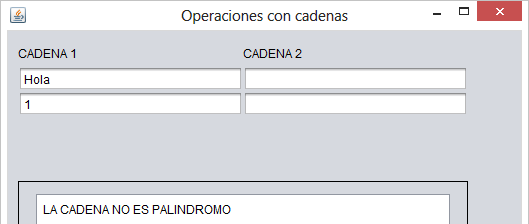
\includegraphics[scale=0.7]{Practica1/Pal_3.PNG}
    	\end{figure}
	\end{itemize}
	\newpage
	\section{Conclusiones}

	Al terminar está práctica pude manejar, diseñar, reafirmar e implementar en un lenguaje de 
	programación las operaciones que se pueden hacer con las cadenas. Con respecto al lenguaje 
	de programación, en mi caso personal jamás había usado estos métodos para trabajar cadenas,
	pero pude ver que es realmente sencillo y práctico usarlos, además de que facilitan mucho el
	trabajo.

	Finalmente las operaciones fueron implementadas de manera correcta y en una interfaz amigable 
	de tal forma que al usuario le fuera fácil trabajar con ellas.

	 \nocite{ref1, ref2}
	\bibliography{referencias}
     
\end{document}